\documentclass[12pt]{article}
\usepackage[utf8]{inputenc}
%\usepackage[portuguese]{babel}
\usepackage{amsmath,amsfonts,amssymb}
\usepackage{graphicx}
\usepackage{makeidx}
\usepackage{graphicx}
\usepackage{lmodern}
\usepackage{multicol}
\usepackage{booktabs}
\usepackage{fancyhdr}
\usepackage{hyperref}
\usepackage[usenames]{color}


\usepackage{Sweave}
\begin{document}
\Sconcordance{concordance:PCA.tex:PCA.Rnw:%
1 15 1 1 0 38 1 1 2 1 0 5 1 1 2 1 1 3 0 1 2 2 1 1 9 1 2 4 1 1 2 1 0 1 4 %
3 0 2 1 1 2 1 1 3 0 1 2 1 1 1 2 1 0 1 2 1 4 6 0 1 2 2 1 1 2 1 0 1 1 1 %
27 29 0 1 2 6 1 1 2 14 0 2 2 3 0 1 1 3 0 1 2 5 1 1 6 1 2 18 1}

\pagestyle{fancy}
\fancyhf{}
\renewcommand{\headrulewidth}{0.4pt}
\fancyfoot[C]{\thepage}
\renewcommand{\footrulewidth}{0.4pt}
\fancyfoot[C]{\thepage}
\title{\LARGE \bf
 Exercício 10 - PCA }
\author{ Rodrigo Machado Fonseca - 2017002253}
\thispagestyle{fancy}
\fancyhead[C]{Introdução ao Reconhecimento de Padrões - UFMG \\ Belo Horizonte - \today}
\maketitle
\thispagestyle{fancy}

%%%%%%%%%%%%%%%%%%%%%%%%%%%%%%%%%%%%%%%%%%%%%%%%%%%%%%%%%%%%%%%%%%%%%%%%%%%%%%%%%%%%%%%%%
\section{Introdução}

  \par Este exercício consiste avaliar o desempenho de um classificador na tarefa de reconhecer imagens de faces humanas.
  
\section{PCA}
  
  \par A técnica de PCA baseia-se em  reduzir a dimensionalidade de um conjunto de dados, preservando o máximo de “variabilidade” (ou seja, informações estatísticas) possível. Diminiur a dimensionalidade implica reduzir a complexidade do sistema, o que acarreta, menos gasto computacional para resolver determinados problemas. Além disso, reduzir a dimensionalidade implica a possibilidade de uma análise visual, o que não seria possível em um espaçõ de alta dimensão. 
  
  \par O algoritmo do PCA baseia-se nos seguintes passos:
  
  \begin{itemize}
    \item Cálcula a média dos dados
    \item Sutrai a média dos dados 
    \item Calcula a matriz de covariância
    \item Encontre os auto-valores e auto vetores
    
  \end{itemize}
  
\section{Experimento}

  \par A priori, carregou-se a base de dados Olivetti. Em sequência, criou-se rótulos para indicar cada uma das classes e aplicou-se o algoritmo PCA.

\begin{Schunk}
\begin{Sinput}
> rm(list=ls())
> library(RnavGraphImageData)
> library(caret)
> library(e1071)
> library(RSNNS)
> set.seed(1)
> data(faces)
> faces <- t(faces)
\end{Sinput}
\end{Schunk}

\begin{figure}[ht]
\centering
\includegraphics{PCA-002}

\caption{Imagem da base Olivetti.}
\label{1}
\end{figure}

\begin{Schunk}
\begin{Sinput}
> nomeColunas <- NULL
> for(i in 1:ncol(faces))
+ {
+   nomeColunas <- c(nomeColunas, paste("a", as.character(i), sep="."))
+ }
> colnames(faces) <- nomeColunas
> rownames(faces) <- NULL
> trans <- preProcess(faces, method = c("BoxCox", "center", "scale", "pca"))
> PC <- predict(trans, faces)
\end{Sinput}
\end{Schunk}

  \par Em sequência selecionou-se as 10 primeiras componentes. Esta base de dados não possui o vetor de rótulos, porém sabemos que cada classe possui 10 amostras e estão dispostas sequencialmente. O código abaixo gera o vetor de rótulos y. Como existem 40 classes o vetor contém valores de rótulos variando entre 1 e 40.
\begin{Schunk}
\begin{Sinput}
> faces <- PC[,(1:10)]
> y <- NULL
> for(i in 1:nrow(faces) )
+ {
+   y <- c( y, ((i-1) %/% 10) + 1 )
+ }
\end{Sinput}
\end{Schunk}

  \par Para relizar  treinar o modelo separou-se 50\% dos dados e o restante para teste. Após isso utilizou-se um classificador bayesiano (\textit{naiveBayes}) e calculou-se a acurácia. Cada experimento foi repetido 10 vezes. 
  
\begin{Schunk}
\begin{Sinput}
> x <- faces
> accuracy_vec <- matrix(nrow = 10, ncol = 1)
> for (k in 1:10)
+ {
+   # Embaralhar dados
+   index <- sample(1:nrow(x), length(1:nrow(x)))
+   x <- x[index,1:ncol(x)]
+   y <- y[index]
+   
+   # Selecionar amostras de teste e treinamento
+   xy_all <- splitForTrainingAndTest(x,y,ratio = 0.5)
+   x_train <- xy_all$inputsTrain
+   y_train <- xy_all$targetsTrain
+   x_test <- xy_all$inputsTest
+   y_test <- xy_all$targetsTest
+   
+   # Classificador de Bayes multivariado
+   model <- naiveBayes(x_train, y_train)
+   y_hat <- predict(model, x_test)
+   
+   accuracy <- 0
+   for(i in 1:length(y_hat) )
+   {
+     score <- if (y_test[i] == y_hat[i]) 1 else 0
+     accuracy <- accuracy + score
+   }
+   accuracy <- accuracy / length(y_test)
+   accuracy_vec[k,] <- accuracy 
+ }
\end{Sinput}
\end{Schunk}

\par Por fim, para a última classficação realizada, gerou-se uma matriz de confusão com os resultados obtidos. Essa matriz de confusão será apresentada na seção seguinte e ela será utilizada para fazer a discussão do desempenho do sistema. A matriz de confusão foi construída por meio da função \textit{conf\_mat} do pacote \textit{yardstick}.

\section{resultados}

  \par Abaixo segue os resutlados da acurácia em cada rodada, a média da acurácia e o desvio padrão, respectivamente.
  
\begin{Schunk}
\begin{Soutput}
      [,1]
 [1,] 62.0
 [2,] 69.5
 [3,] 67.5
 [4,] 65.5
 [5,] 66.0
 [6,] 67.5
 [7,] 63.5
 [8,] 56.0
 [9,] 59.5
[10,] 63.5
\end{Soutput}
\end{Schunk}

\begin{Schunk}
\begin{Soutput}
[1] 0.6405
\end{Soutput}
\begin{Soutput}
[1] 0.04078739
\end{Soutput}
\end{Schunk}


\par Em sequência, a figura \ref{1} abaixo apresenta os resultados da última classificação na forma de matriz de confusão.

\begin{figure}[ht]
\centering
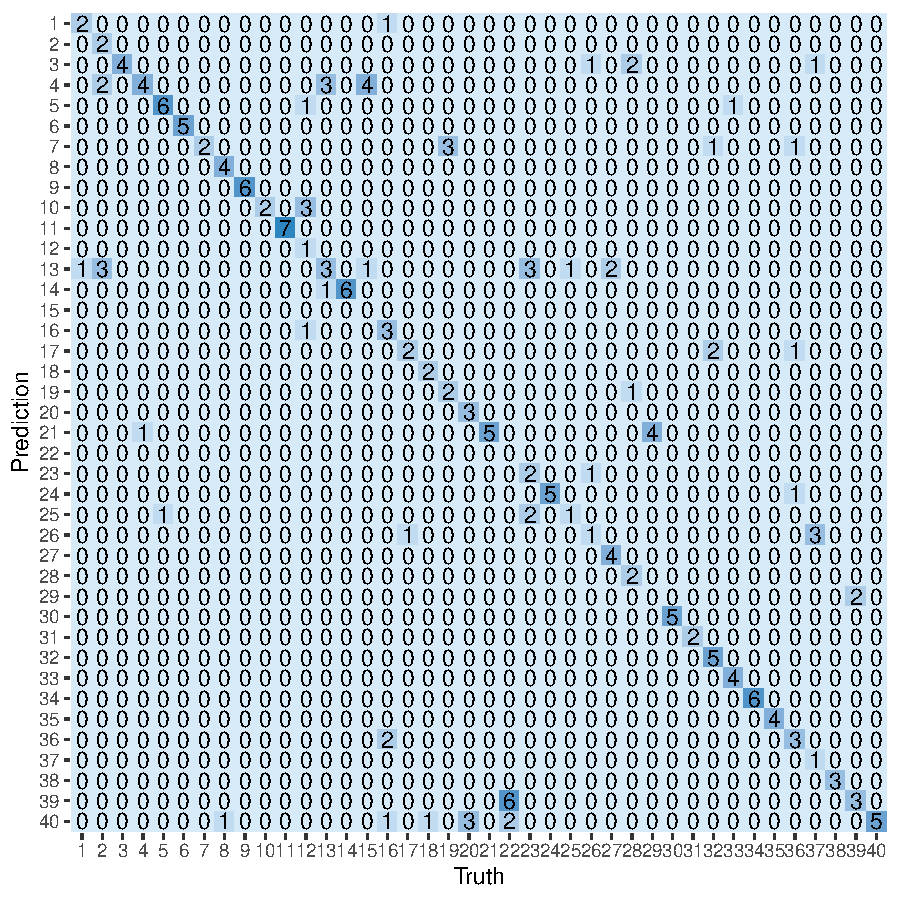
\includegraphics{PCA-008}
\caption{Matriz de confusão dos resultados do classificador de Bayes}
\label{1}
\end{figure}

\section{Discussão}

  \par Após o experimento, pode-se observar que a utilização de apenas 10 componentes principais não obteve resultados satisfatório. Uma alternativa é aumentar o número de componentes principais e analisar os resultados. 
  
  \par A matriz de confusão mostra os elementos e suas classsificações. Pode-se observar que algumas amostras são projetadas em cima de outras classes, por exemplo a 39, em que 6 amostras foram classsificadas sobre a classe 22. Além disos, podemos observar que não havia nenhuma amostra da classe 22 naquela rodada. 
  
  \par Embora os resultados obtidos foram abaixo do esperado, foi possível avaliar o algoritmo PCA e utilizá-lo em conjunto com classificador de Bayes. 

%%%%%%%%%%%%%%%%%%%%%%%%%%%%%%%%%%%%%%%%%%%%%%%%%%%%%%%%%%%%%%%%%%%%%%%%%%%%%%%%%%%%%%%%%

%%%%%%%%%%%%%%%%%%%%%%%%%%%%%%%%%%%%%%%%%%%%%%%%%%%%%%%%%%%%%%%%%%%%%%%%%%%%%%%%%%%%%%%%%



\end{document}
